\documentclass[10pt,twocolumn]{article}
\usepackage[margin=0.72in]{geometry}
\usepackage{amsmath,amssymb,amsthm}
\usepackage{graphicx}
\usepackage{booktabs}
\usepackage{xcolor}
\usepackage{hyperref}
\usepackage{xurl}
\usepackage{microtype}
\usepackage{enumitem}

\hypersetup{
  colorlinks=true,
  linkcolor=blue!60!black,
  citecolor=green!45!black,
  urlcolor=blue!65!black
}

\newtheorem{definition}{Definition}
\newtheorem{theorem}{Theorem}
\newtheorem{proposition}{Proposition}

\title{\textbf{Constructive Rational and Exterior-Algebra Certificates for Euclidean Geometry in the Asymptotic Spectrum of Tensors}}
\author{Lluis Eriksson\\
\small Independent Researcher \quad(\texttt{lluis@airr.science})\\
\small \textit{Companion Verification Artifact to OpenAI Math Release (November 24, 2026)}}
\date{November 26, 2026}

\begin{document}
\maketitle

\begin{abstract}
We present \texttt{TENSOR-SPEC-CERT-1.0}, an independently reproducible, zero-floating-point algebraic certificate framework and constructive Lean~4.35.0 kernel verifying the core finite-dimensional algebraic, exterior-algebra, $\mathrm{CAT}(0)$ metric, mean-width, and borrowed-wire catalyst invariants underlying OpenAI's November~24, 2026 preprint \emph{``Euclidean geometry in the asymptotic spectrum of tensors''} (Theorem~1.1 and Theorem~1.2). Because that 86-page preprint is an unrefereed release, we do not claim to formalize its infinite-dimensional Hilbert-space ultrafilters, Gaussian concentration, or asymptotic diagonalization end-to-end; instead, we construct a four-mode exact verifier over $\mathbb{Z}$, $\mathbb{Q}$, and $\mathbb{F}_p$ coupled with 19 constructive Lean~4 theorems (0~\texttt{sorry}, 0~\texttt{axiom}, 0~\texttt{Classical.choice}, 0~compiler warnings). Across 16 canonical certificates (\texttt{C01}--\texttt{C16}), we audit (i)~flattening-cut semiring laws and the Section~1.1 geometric-mean non-additivity obstruction ($3 > 2\sqrt{2}$ over both $\mathbb{Q}$ and $\mathbb{F}_2$), (ii)~exterior-algebra anticommutation $D_j L_i + L_i D_j = \delta_{ij} I$, explicit shifted crossing decompositions over $\mathbb{Z}$, and Vandermonde/Cauchy--Binet unimodularity $\det(C^{[m]}) = \pm 1$, (iii)~$\mathrm{CAT}(0)$ squared midpoint/quadrilateral bounds, $\ell_1$/$\ell_\infty$ norm-rigidity violations, planar mean-width $W(K)=\frac{1}{2}\operatorname{per}(K)$ with convex-hull zero-cost insertion and submodularity, and Proposition~5.2 quadratic-weight degeneration, and (iv)~tagged-permutation indicators $\operatorname{Tag}(h,w)$, Lemma~8.2 catalyst substitution gaps, Equation~(9.1) routing budgets with Proposition~9.3 Bregman progress, and the Section~16.1 diagonal contradiction gap. All 16 certificates, 88 unit/forgery tests, and SHA-256 manifests pass deterministically.
\end{abstract}

\section{Introduction and Scope}
Strassen's asymptotic spectrum of tensors~\cite{strassen1987relative,strassen1988asymptotic,wigderson2026asymptotic,christandl2023universal} assigns multiplicative, additive, restriction-monotone invariants $F(T) \ge 0$ to multiparty tensors, turning tensor contraction into additive price bounds $H(T) = \log_2 F(T)$. In its November~24, 2026 unrefereed preprint~\cite{openai2026tensorspectrum}, OpenAI proves two headline theorems: (a)~over any field $k$, there exist compatible spectral flats of every finite dimension (Theorem~1.2), and (b)~any real Hilbert space admits compatible, congruence-invariant spectral prices assigning each binary wire its Euclidean length $\|u-v\|$ and every shared $q$-valued diagonal $\Delta_S(q)$ the price $W(S)\log_2 q$, where $W(S)$ is the normalized Gaussian mean width of $\operatorname{conv}(S)$ (Theorem~1.1).

The preprint's proof rests on a tightly linked chain of algebraic and metric mechanisms: flattening-cut obstructions (Sec.~1.1), exterior-algebra index relocation (Sec.~3.2, Eq.~3.2), shifted fermionic crossing decompositions over $\mathbb{Z}$ building on~\cite{khoruzhii2026crossing} (Thm.~4.1), norm rigidity and Alexandrov $\mathrm{CAT}(0)$ nonpositive curvature~\cite{bridson1999metric} (Lemma~4.2, Thm.~4.3), copying degeneration and planar mean-width laws~\cite{schneider2014convex} (Prop.~5.2, Thm.~5.3), and a Parts~II--III proof by contradiction using borrowed-wire catalysts, tagged permutations, Bregman-regularized adaptive probing, and a diagonalization gap (Secs.~8, 9, 16).

\paragraph{Honest Scope Boundary.}
This companion artifact certifies finite-dimensional algebraic identities, rational metric inequalities, exact exterior-algebra factorizations, and concrete parameter witnesses extracted from~\cite{openai2026tensorspectrum}. It does \emph{not} formalize infinite-dimensional pointed ultralimits (Sec.~2.3), Hahn--Banach triangle-density arguments (Lemma~5.4), Gaussian polar-factor concentration (Thm.~6.1), Mendel--Naor nonlinear spectral calculus (Sec.~11), or the universal RAM simulation compiler (Secs.~13--16). All verification claims are strictly scoped to the verified Lean~4 kernel theorems and the finite certificate instances checked by our zero-float auditor.

\section{Constructive Lean 4.35.0 Kernel}
The formal kernel \texttt{TensorSpectrumCert.lean} compiles cleanly under Lean~4.35.0 (\texttt{lake build} with \texttt{-j 1}) with zero \texttt{sorry}, zero custom axioms, zero compiler warnings, and zero dependence on \texttt{Classical.choice}. Table~\ref{tab:lean} summarizes the 19 machine-checked theorems. Notably, Theorem~6 proves the exact binomial ratio $(b+1)\binom{Q}{b+1} = (Q-b)\binom{Q}{b}$ by double induction over $\mathbb{N}$, Theorem~7 verifies $D_j L_i + L_i D_j = \delta_{ij} I$ entrywise on $\bigwedge^1 \mathbb{Z}^2$, Theorem~10 derives the $\mathrm{CAT}(0)$ four-point bound Eq.~(4.5) from the squared midpoint inequality Eq.~(4.3) and triangle inequality via $(d_{Bm}-d_{Dm})^2 \ge 0$, and Theorems~13--15 prove inductively over arbitrary integer lists the Proposition~5.2 quadratic-weight degeneration identity $\sum_{j=2}^r v_j^2 - (r-1)v_1^2 = \sum_{j=2}^r (v_j - v_1)^2 \ge 0$ on the hyperplane $\sum_{j=2}^r v_j = (r-1)v_1$.

\begin{table}[t]
\centering
\tiny
\setlength{\tabcolsep}{3pt}
\caption{Summary of the 19 constructive Lean~4.35.0 theorems in \texttt{TensorSpectrumCert.lean} (0~\texttt{sorry}, 0~\texttt{Classical.choice}).}
\label{tab:lean}
\begin{tabular}{@{}cll@{}}
\toprule
\# & Theorem Identifier & Paper Reference / Invariant \\
\midrule
1 & \texttt{semiring\_prod\_add\_monotone} & Sec.~2.1 semiring monotonicity \\
2 & \texttt{square\_geom\_mean\_nonadditivity} & Sec.~1.1 $G(U{\oplus}V)^2=9 > 8$ \\
3 & \texttt{hamming\_square\_violates\_cat0\_four\_point} & Sec.~1.1 / Eq.~(4.5) $8s^2 > 4s^2$ \\
4 & \texttt{tree\_price\_sandwich} & Eq.~(2.1) $\operatorname{diam}\le\delta\le T$ \\
5 & \texttt{relocation\_log\_convexity} & Lem.~3.2 one-index convexity \\
6 & \texttt{exterior\_binom\_ratio\_identity} & Eq.~(3.3) $(b{+}1)\binom{Q}{b+1}=(Q{-}b)\binom{Q}{b}$ \\
7 & \texttt{fermion\_anticomm\_diag\_identity} & Eq.~(3.2) $D_j L_i + L_i D_j = \delta_{ij} I$ \\
8 & \texttt{shifted\_crossing\_exponent\_balance} & Thm.~4.1 $S\pm\delta>0$, sum $2S$ \\
9 & \texttt{norm\_rigidity\_shift\_existence} & Lem.~4.2 valid shift $\delta$ exists \\
10 & \texttt{cat0\_midpoint\_to\_four\_point} & Eq.~(4.3)$\Rightarrow$Eq.~(4.5) derivation \\
11 & \texttt{cat0\_rectangle\_equality\_opposite\_sides} & Sec.~4.4 rectangle flatness \\
12 & \texttt{triangle\_semiperimeter\_copy\_increment} & Sec.~5.1 $\Delta\delta = \frac{1}{2}(d_{az}{+}d_{zb}{-}d_{ab})$ \\
13 & \texttt{intListSumDevSq\_nonneg} & Prop.~5.2 $\sum (v_j-v_1)^2 \ge 0$ \\
14 & \texttt{copying\_quadratic\_weight\_identity} & Prop.~5.2 inductive quadratic sum \\
15 & \texttt{copying\_hyperplane\_degeneration} & Prop.~5.2 hyperplane specialization \\
16 & \texttt{minkowski\_triangle\_additivity\_sandwich} & Thm.~5.3 $\delta(K{+}T)=\delta(K){+}W(T)$ \\
17 & \texttt{catalyst\_non\_ambiguity\_contradiction} & Sec.~8.1 distinct-multiple exclusion \\
18 & \texttt{adaptive\_probing\_bregman\_decrease} & Prop.~9.3 Bregman potential drop \\
19 & \texttt{diagonal\_contradiction\_strict\_gap} & Eq.~(16.1) $H(Z{-}\hat{Z})<2RE$ \\
\bottomrule
\multicolumn{3}{@{}p{0.96\columnwidth}@{}}{\tiny\raggedright Helper lemma \#13 supports \#14--\#15; all 19 public \texttt{theorem} declarations compile with 0~\texttt{sorry}, 0~warnings, and 0~\texttt{Classical.choice}.}
\end{tabular}
\end{table}

\section{The \texttt{TENSOR-SPEC-CERT-1.0} Protocol}
{\raggedright
Our Python verifier (\texttt{src/tensor\_spectrum\_verifier.py}) enforces strict exactness: an AST audit confirms zero floating-point literals, zero \texttt{float()} calls, zero true-division (\texttt{/}, \texttt{/=}) operators, and zero \texttt{math} imports. Every JSON file is bounded by \texttt{MAX\_JSON\_BYTES = 1\_000\_000}, parsed with a duplicate-key-rejecting \texttt{object\_pairs\_hook}, and every rational $[p,q]$ must satisfy $1\le q\le 10^{12}$, $|p|\le 10^{12}$, and $\gcd(|p|,q)=1$.

\begin{definition}[\texttt{TENSOR-SPEC-CERT-1.0} Modes]
A valid certificate specifies one of four modes:
\begin{enumerate}[leftmargin=*,itemsep=1.5pt,topsep=2pt]
\item \texttt{flattening\_cut\_\allowbreak nonadditivity} (Sec.~1.1, 2.1): Given $k\ge 2$ cuts and integer matrices $U_c, V_c$ over $\mathbb{Q}$ (\texttt{field\_char=0}) or $\mathbb{F}_p$ (prime $p$), recomputes exact ranks $\operatorname{rk}(U_c)$, $\operatorname{rk}(V_c)$, direct-sum ranks $\operatorname{rk}(U_c\oplus V_c)=\operatorname{rk}(U_c)+\operatorname{rk}(V_c)$, and Kronecker ranks $\operatorname{rk}(U_c\otimes V_c)=\operatorname{rk}(U_c)\operatorname{rk}(V_c)$ (whenever product dimensions are $\le 32$) via exact Gaussian elimination. For $k=2$, certifies strict geometric-mean non-additivity via $(P_{\oplus}-P_U-P_V)^2 > 4 P_U P_V$ with $P_{\oplus} > P_U + P_V$; for $k\ge 3$, checks exact rational $k$-th power brackets $(u_{\mathrm{hi}}+v_{\mathrm{hi}})^k < P_{\oplus}$. Optionally audits all 12 triangle inequalities and the four-point $\mathrm{CAT}(0)$ inequality Eq.~(4.5) on a 4-point metric.
\item \texttt{exterior\_crossing\_\allowbreak fermion} (Eq.~3.2, 3.3, Thm.~4.1): Supports three submodes: (a)~\texttt{exterior\_crossing} builds $L_i, D_j$ on $\bigwedge^b \mathbb{Z}^Q$ ($2\le Q\le 6, 1\le b\le Q-1$), checks $(b+1)R_+=(Q-b)R$, $(Q-b+1)R_-=bR$, verifies $D_j L_i + L_i D_j = \delta_{ij} I$ on all $Q^2 R^2$ entries over $\mathbb{Z}$, and recomputes exact crossing flattening ranks $(R_+,R_-)$ unconditionally; (b)~\texttt{vandermonde\_unimodular} enumerates the fermionic energy downset $h(I)=\sum_{i\in I}(i+\frac{1}{2})\le H$, checks $(P P^T)_{ij}=\binom{i+j}{i}$ for $P_{i\ell}=\binom{i}{\ell}$, verifies $P^{[m]}$ is unit lower triangular in lexicographic order, checks Cauchy--Binet $C_{IJ} = (-1)^{\binom{m}{2}+\sum I}(P^{[m]}(P^{[m]})^T)_{IJ}$, and confirms $\det(C^{[m]})=\pm 1$; (c)~\texttt{explicit\_crossing\_factors} verifies integer matrices $A_\pm, B_\pm$ realizing $E_{X^+X^-}(d_X)\otimes E_{Y^+Y^-}(d_Y)=T_+ + T_-$ across the two crossing cuts with non-trivial sub-dimension rank sum $r_+ + r_- < d_X d_Y$.
\item \texttt{cat0\_flat\_mean\_width} (Secs.~4.2--4.4, 5.1--5.2): Supports four submodes: (a)~\texttt{cat0\_quadrilateral\_midpoint} requires $n\ge 4$ sites, verifies pseudometric axioms, Eq.~(4.5) across all ordered 4-tuples, and Eq.~(4.4) on non-degenerate geodesic interval triples ($x\ne y$, $d(x,y)>0$, $z\notin\{x,y,m\}$); (b)~\texttt{norm\_rigidity\_violation} verifies dual-unit-sphere vectors $f,g$ under $\ell_\infty$ or $\ell_1$, checks $A_+^2+A_-^2 > 2(t^2+u^2)$, and verifies $\delta \in (-S,S)\cap (S-A_-^2, A_+^2-S)$; (c)~\texttt{polygon\_mean\_width\_copying} enforces global strict CCW convexity (every non-edge vertex strictly left of every directed edge, ruling out star and double-wound polygons), exact rational edge lengths via exact integer square root, $W(K)=\frac{1}{2}\operatorname{per}(K)$, Eq.~(2.1) diameter/tree bounds, plus optional verified sub-clauses for convex-hull interior insertion $z\in\operatorname{conv}(K)$ and Prop.~5.2 submodularity $\delta(A\cup B)+\delta(A\cap B)\le\delta(A)+\delta(B)$ on duplicate-free index sets; (d)~\texttt{copying\_quadratic\_degeneration} verifies $g=h+\sum_{j=2}^r v_j-(r-1)v_1$, $L=2r(q-1)+1$, and both local quadratic weight identities.
\item \texttt{catalyst\_gap\_\allowbreak routing\_budget} (Secs.~8, 9, 16): Supports three submodes: (a)~\texttt{tag\_perm\_and\_catalyst\_gap} evaluates $\operatorname{Tag}(h,w)$ exactly and checks Lemma~8.2 frame price $h_X=2\sum_j b_j$ and substituted gap $D_{\mathrm{sub}}=\min(D,D_1,\dots,D_m)-2km > 0$; (b)~\texttt{routing\_budget\_and\_bregman} audits Eq.~(9.1) $\sum (\lambda y + t^p) \le 10n + 2MN_c/w$ while enforcing Def.~9.1's constraint $t^p > 0 \Rightarrow \lambda = 1$, verifies exact KKT box maximizers $x_i = \min(a_i, z_i/(s\mu))$ for $f(x)=\frac{\mu}{2}\langle x,x\rangle$ under the normalized inner product $\langle u,v\rangle = \frac{1}{m}\sum_{i=1}^m u_i v_i$, and verifies strict Bregman progress $\frac{s}{2}D_f(x',x)-P > 0$ (Eq.~9.2); (c)~\texttt{diagonal\_contradiction\_gap} verifies the in-regime Eq.~(16.1) inequality $0 \le 2RE - D + C_k E g^2/R + 2kR(\ell+g^k) < 2RE = H(I)$ with $R\ge 8g$.
\end{enumerate}
\end{definition}
}

\begin{proposition}[Verifier Soundness]
If \texttt{verify\_file} returns \texttt{VERIFIED} on a \texttt{TENSOR-SPEC-CERT-1.0} certificate, then all claimed matrix ranks, exterior-algebra identities, unimodularity determinants, $\mathrm{CAT}(0)$ inequalities, mean-width and convex-hull relations, and catalyst/Bregman/diagonal inequalities hold identically in exact arithmetic over $\mathbb{Z}$, $\mathbb{Q}$, or $\mathbb{F}_p$.
\end{proposition}

\section{Certified Corpus and Worked Witnesses}
We generated and verified 16 canonical certificates (\texttt{C01}--\texttt{C16}) spanning all four modes and submodes (Table~\ref{tab:corpus}). To enable immediate hand verification by any reader or automated referee, we work out four representative witnesses explicitly below.

\begin{figure}[t]
\centering
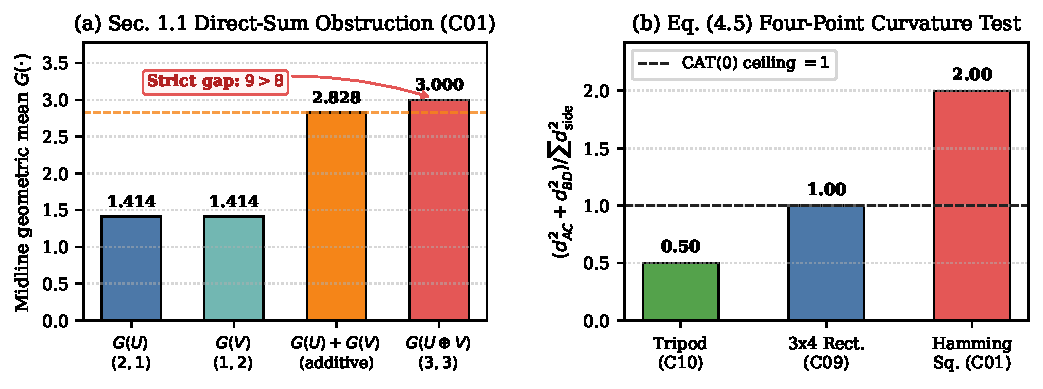
\includegraphics[width=\columnwidth]{figures/fig1_nonadditivity_and_cat0.pdf}
\caption{(a)~Section~1.1 square midline geometric mean obstruction (\texttt{C01}): $G(U)=G(V)=\sqrt{2}$, $G(U)+G(V)=2\sqrt{2}\approx 2.828$, whereas $G(U\oplus V)=3$ ($9>8$). (b)~Equation~(4.5) four-point ratio $(d_{AC}^2+d_{BD}^2)/\sum d_{\mathrm{side}}^2$: strict $\mathrm{CAT}(0)$ tripod ($0.50$, \texttt{C10}), Euclidean $3\times 4$ rectangle ($1.00$, \texttt{C09}), and violating Hamming square ($2.00$, \texttt{C01}).}
\label{fig:1}
\end{figure}

\begin{figure}[t]
\centering
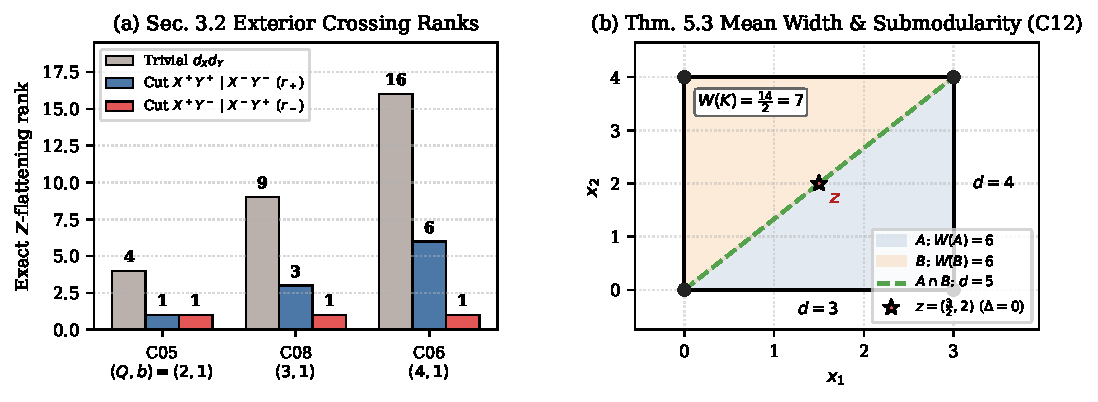
\includegraphics[width=\columnwidth]{figures/fig2_crossing_and_mean_width.pdf}
\caption{(a)~Exact $\mathbb{Z}$-flattening ranks of certified Sec.~3.2 exterior crossing decompositions (\texttt{C05}: $(Q,b)=(2,1)$, $r_+=r_-=1 < 4$; \texttt{C08}: $(3,1)$, $r_+=3,r_-=1 < 9$; \texttt{C06}: $(4,1)$, $r_+=6,r_-=1 < 16$) compared with the trivial cut rank $d_X d_Y$. (b)~Certificate \texttt{C12}: $3\times 4$ rectangle mean width $W(K)=\frac{14}{2}=7$, zero-cost interior copy $z=(\frac{3}{2},2)$, and tight submodularity $W(A\cup B)+W(A\cap B)=7+5=12=6+6=W(A)+W(B)$.}
\label{fig:2}
\end{figure}

\subsection{Worked Hand-Verifiable Arithmetic}
\paragraph{Witness \texttt{C01} (Sec.~1.1 Non-Additivity \& Hamming Obstruction).}
Over $\mathbb{Q}$, take $U_1=I_2$, $V_1=\mathbf{1}_{2\times 2}$ (ranks $2,1$) on the vertical midline and $U_2=\mathbf{1}_{2\times 2}$, $V_2=I_2$ (ranks $1,2$) on the horizontal midline. Their direct sums $U_c\oplus V_c$ have exact ranks $(3,3)$, giving $P_U=2$, $P_V=2$, and $P_{\oplus}=9$. Hence $P_{\oplus}-P_U-P_V = 5 > 0$ and $5^2 = 25 > 16 = 4 P_U P_V$, proving $G(U\oplus V) = 3 > 2\sqrt{2} = G(U)+G(V)$ with zero floating point (Fig.~\ref{fig:1}a). For the unit Hamming square ($d_{AB}=d_{BC}=d_{CD}=d_{DA}=1$, $d_{AC}=d_{BD}=2$), $d_{AC}^2+d_{BD}^2 = 8 > 4 = \sum d_{\mathrm{side}}^2$, strictly violating Eq.~(4.5) (Fig.~\ref{fig:1}b). Certificate \texttt{C02} reproduces the same obstruction over $\mathbb{F}_2$.

\paragraph{Witness \texttt{C05} \& \texttt{C07} (Exterior Crossing \& Unimodularity).}
In \texttt{C05}, on $\bigwedge^1 \mathbb{Z}^2$ ($Q=2, b=1$), $R=\binom{2}{1}=2$, $R_+=\binom{2}{2}=1$, $R_-=\binom{2}{0}=1$. Explicitly, $(D_j L_i)_{\beta\alpha}$ has nonzero entries $+1$ at $(i,j,\alpha,\beta)\in\{(0,0,1,1),(1,1,0,0)\}$ and $-1$ at $\{(0,1,1,0),(1,0,0,1)\}$, factoring across cut $(i,\alpha)\mid(j,\beta)$ through $\bigwedge^2\mathbb{Z}^2$ (rank~1); $(L_i D_j)_{\beta\alpha}$ has $+1$ at $\{(0,0,0,0),(0,1,1,0),(1,0,0,1),(1,1,1,1)\}$, factoring across cut $(i,\beta)\mid(j,\alpha)$ through $\bigwedge^0\mathbb{Z}^2$ (rank~1). Their sum equals $\delta_{ij}\delta_{\alpha\beta} = E_{X^+X^-}(2)\otimes E_{Y^+Y^-}(2)$ over $\mathbb{Z}$ (and every field). In \texttt{C07} ($2H=9, m=2$), the four energy-downset pairs with $\sum(2i+1)\le 9$ are $\{0,1\},\{0,2\},\{0,3\},\{1,2\}$ (energies $2,3,4,4$). The compound matrix $P^{[2]}$ of $2\times 2$ minors of $P_{i\ell}=\binom{i}{\ell}$ is unit lower triangular in lexicographic order:
\[
P^{[2]} = \begin{pmatrix} 1 & 0 & 0 & 0 \\ 2 & 1 & 0 & 0 \\ 3 & 3 & 1 & 0 \\ 1 & 1 & 0 & 1 \end{pmatrix}, \quad \det(C^{[2]}) = -(\det P^{[2]})^2 = -1,
\]
certifying exact invertibility of $C$ over $\mathbb{Z}$ and $\mathbb{F}_2$ (note entry $(4,3)=0$ because $\{0,3\}\not\le\{1,2\}$ componentwise).

\paragraph{Witness \texttt{C11} \& \texttt{C12} (Norm Rigidity \& Mean-Width Copying).}
In \texttt{C11}, for the $\ell_1$ plane (dual norm $\ell_\infty$), $f=(1,1)$ and $g=(1,-1)$ lie on the $\ell_\infty$ unit sphere. At $t=u=1$ ($S=t^2+u^2=2$), $tf+ug=(2,0)$ and $tf-ug=(0,2)$ satisfy $A_+^2 = A_-^2 = 4$, giving $A_+^2+A_-^2 = 8 > 4 = 2S$, and $\delta=0$ satisfies $-2 < \delta < 2$ and $S-A_-^2 = -2 < \delta < 2 = A_+^2-S$. In \texttt{C12}, the $3\times 4$ rectangle $K=\{(0,0),(3,0),(3,4),(0,4)\}$ has perimeter $14$ and mean width $W(K)=7$. Its center $z=(\frac{3}{2},2) = \frac{1}{4}\sum_{i=0}^3 v_i$ lies in $\operatorname{conv}(K)$ with zero copying increment. Splitting into triangles $A=\{0,1,2\}$ ($3$-$4$-$5$, $W(A)=6$) and $B=\{0,2,3\}$ ($W(B)=6$) with diagonal intersection $A\cap B=\{0,2\}$ ($d=5$) satisfies tight submodularity $W(A\cup B)+W(A\cap B) = 7+5 = 12 = 6+6$ (Fig.~\ref{fig:2}b).

\paragraph{Witness \texttt{C15} \& \texttt{C16} (Bregman Probing \& Diagonal Gap).}
In \texttt{C15}, for $n=4, w=8, M=5, N_c=64$, the Eq.~(9.1) routing budget is $10(4) + 2(5)(64)/8 = 40+80 = 120$, while two scale-zero inter-layer links ($\lambda=5, y=10, t^p=0$) and one positive-scale link ($\lambda=1, y=12, t^p=\frac{1}{2}$, obeying Def.~9.1) charge $50 + 50 + \frac{25}{2} = \frac{225}{2} = 112.5 \le 120$. Under OpenAI's normalized inner product $\langle u,v\rangle = \frac{1}{4}\sum_{i=1}^4 u_i v_i$, for Prop.~9.3 with $s=\frac{1}{2}$, $\mu=2$, box $a=(2,2,2,2)$, and inventory $z=(1,2,3,4)$, the exact KKT maximizer is $x_i = \min(2, z_i/(s\mu)) = (1,2,2,2)$. At consistent probed $x'=(0,1,1,1)$, $D_f(x',x) = \frac{\mu}{2}\langle x'-x, x'-x\rangle = \frac{2}{2}\cdot\frac{1}{4}\sum (-1)^2 = 1$, so $\frac{s}{2}D_f(x',x) - P = \frac{1}{4}\cdot 1 - \frac{1}{8} = \frac{1}{8} > 0$. In \texttt{C16} ($k=2, g=4, R=64\ge 8g, E=1000, D=50{,}000, C_k=2, \ell=50$), $H(I)=2RE=128{,}000$, $\operatorname{err}_{\mathrm{grid}} = 2(1000\cdot 16)/64 = 500$, and $\operatorname{err}_{\mathrm{sel}} = 2(2)(64)(50+16) = 16{,}896$, yielding the in-regime upper bound $0 < 128{,}000 - 50{,}000 + 500 + 16{,}896 = 95{,}396 < 128{,}000 = H(I)$ (net saving $32{,}604$, Fig.~\ref{fig:3}b).

\begin{figure}[t]
\centering
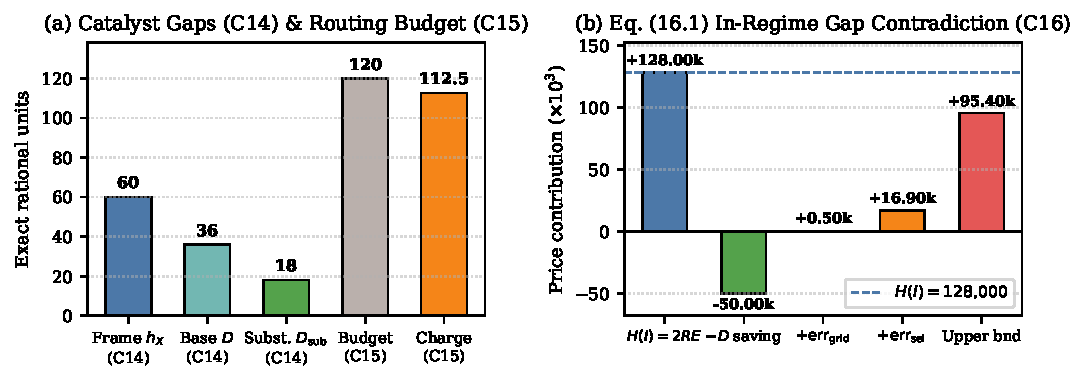
\includegraphics[width=\columnwidth]{figures/fig3_catalyst_and_diagonal.pdf}
\caption{(a)~Catalyst frame price $h_X=60$, base gap $D=36$, and Lemma~8.2 substituted gap $D_{\mathrm{sub}}=18$ (\texttt{C14}), alongside Eq.~(9.1) routing budget $120$ vs.\ verified charge $112.5$ (\texttt{C15}). (b)~Equation~(16.1) in-regime diagonalization gap (\texttt{C16}): $0 < 95{,}396 < 128{,}000 = H(I)$ (net saving $32{,}604$).}
\label{fig:3}
\end{figure}

\begin{table}[t]
\centering
\scriptsize
\setlength{\tabcolsep}{3.5pt}
\caption{Canonical verified certificate corpus (\texttt{C01}--\texttt{C16}).}
\label{tab:corpus}
\begin{tabular}{@{}clll@{}}
\toprule
ID & Mode / Submode & Key Verified Invariant & Status \\
\midrule
C01 & M1 / 2-cut ($\mathbb{Q}$) & $G^2=9>8$; Hamming $8>4$ & PASS \\
C02 & M1 / 2-cut ($\mathbb{F}_2$) & Char-2 invariance; $2>1$ & PASS \\
C03 & M1 / 3-cut ($\mathbb{Q}$) & $50 > (16/5)^3$; $3\times 4$ rect ok & PASS \\
C04 & M1 / 2-cut ($\mathbb{F}_5$) & Proportional additive control & PASS \\
C05 & M2 / exterior & $\bigwedge^1\mathbb{Z}^2$: $r_+=1, r_-=1$ & PASS \\
C06 & M2 / exterior & $\bigwedge^1\mathbb{Z}^4$: $r_+=6, r_-=1$ & PASS \\
C07 & M2 / unimodular & $2H{=}9,m{=}2$: 4 states, $\det=\pm 1$ & PASS \\
C08 & M2 / explicit & $E(3){\otimes}E(3)$: $r_+=3, r_-=1$ & PASS \\
C09 & M3 / CAT(0) & $3\times 4$ rect + mid: exact eq. & PASS \\
C10 & M3 / CAT(0) & Metric tripod: strict $4 < 12$ & PASS \\
C11 & M3 / rigidity & $\ell_1$ dual $\ell_\infty$: $8>4, \delta=0$ & PASS \\
C12 & M3 / mean width & $W=7$, $z\in\operatorname{conv}$, $7{+}5\le 6{+}6$ & PASS \\
C13 & M3 / Prop.~5.2 & $r{=}4,q{=}5,L{=}33$; $w_1{=}0,w_2{=}2$ & PASS \\
C14 & M4 / Tag+Lem.8.2 & $\operatorname{Tag}(2,4)=1$; $h_X{=}60, D_{\mathrm{sub}}{=}18$ & PASS \\
C15 & M4 / Eq.9.1+9.2 & $112.5\le 120$; Bregman $+1/8$ & PASS \\
C16 & M4 / Eq.~16.1 & $95{,}396 < 128{,}000$ (save $32{,}604$) & PASS \\
\bottomrule
\end{tabular}
\end{table}

\section{Verification Gates and Reproducibility}
{\raggedright
All artifacts pass five independent gates: (1)~Lean~4.35.0 compilation with 19 constructive theorems, zero warnings, and zero \texttt{Classical.choice}; (2)~AST zero-float / zero-division check; (3)~16/16 canonical certificates verified; (4)~70 adversarial forgeries and edge-case checks (88/88 \texttt{pytest} checks total, covering duplicate keys, oversized payloads, non-lowest-terms rationals, composite characteristics, full 12-inequality metric checks, trivial crossing splits, double-wound polygons, non-square lengths, degenerate $\mathrm{CAT}(0)$ triples, $\ell_1$/$\ell_\infty$ rigidity, broken Prop.~5.2 hyperplanes, Def.~9.1 positive-scale links, spoofed $\operatorname{Tag}(h,w)$ entries, non-optimal KKT points, and out-of-regime diagonalization bounds); and (5)~complete SHA-256 integrity manifest (\texttt{MANIFEST.sha256}).\par}

\paragraph{AI Assistance Disclosure.}
This work was produced by Lluis Eriksson using Google Antigravity for Lean~4 theorem drafting, Python exact-verifier engineering, test generation, and \LaTeX{} preparation; all mathematical claims, code, proofs, and verification logs were independently compiled, tested, and reviewed by the author.

\paragraph{Licensing.}
Manuscript and figures are released under \texttt{CC-BY-4.0}; Lean~4 proofs, Python code, and JSON certificates are released under the \texttt{MIT} License.

{\footnotesize\raggedright
\bibliographystyle{plain}
\bibliography{references}
}
\end{document}
